\section{Results}
We consider Keplerian disks so that $S = 1.5$ and $\kappa = \Omega =
\Omega_z.$ In the linear simulations below we fix $\beta=100$ and the
vertical extent of the disk is $Z_s=0.99$ and $Z_s=1$ in the
polytropic and isothermal disk, respectively. The numerical resolution
is $N_z=256$.  


\subsection{MRI in self-gravitating polytropic disks with uniform
  resistivity}  
We first calculate the MRI as a function of $Q$ in a polytropic disk
with uniform resistivity ($A=1$). We consider $Q\in[0.2,4]$,
corresponding to stronly self-gravitating to non-self-gravitating
disks, for mid-plane Elsasser numbers $\Lambda_0\in[0.3,10]$. We fix
$k_x=0.1$.  
%We fix $k_x=0.1$ and $\beta=100$. The disk vertical extent is
%$Z_s=0.99$ and adopt a numerical resolution of $N_z=256$. 

Fig. \ref{compare_growth_poly_uniresis} plots the MRI growth rates as
a function of $Q$ and $\Lambda_0$. As expected growth rates generally
decrease with $\Lambda_0$. In the limit of ideal MHD, $\Lambda_0>1$,
there is negligible dependence on $Q$. In the resistive limit,
$\Lambda_0<1$, growth rates decrease noticeably for $Q<1$. This shows
show that self-gravity can still affect the MRI even  
though density and potential perturbations are expected to be
negligible because $k_x\ll1$ (i.e. the linear response is
non-self-gravitating).    
 
\begin{figure}
  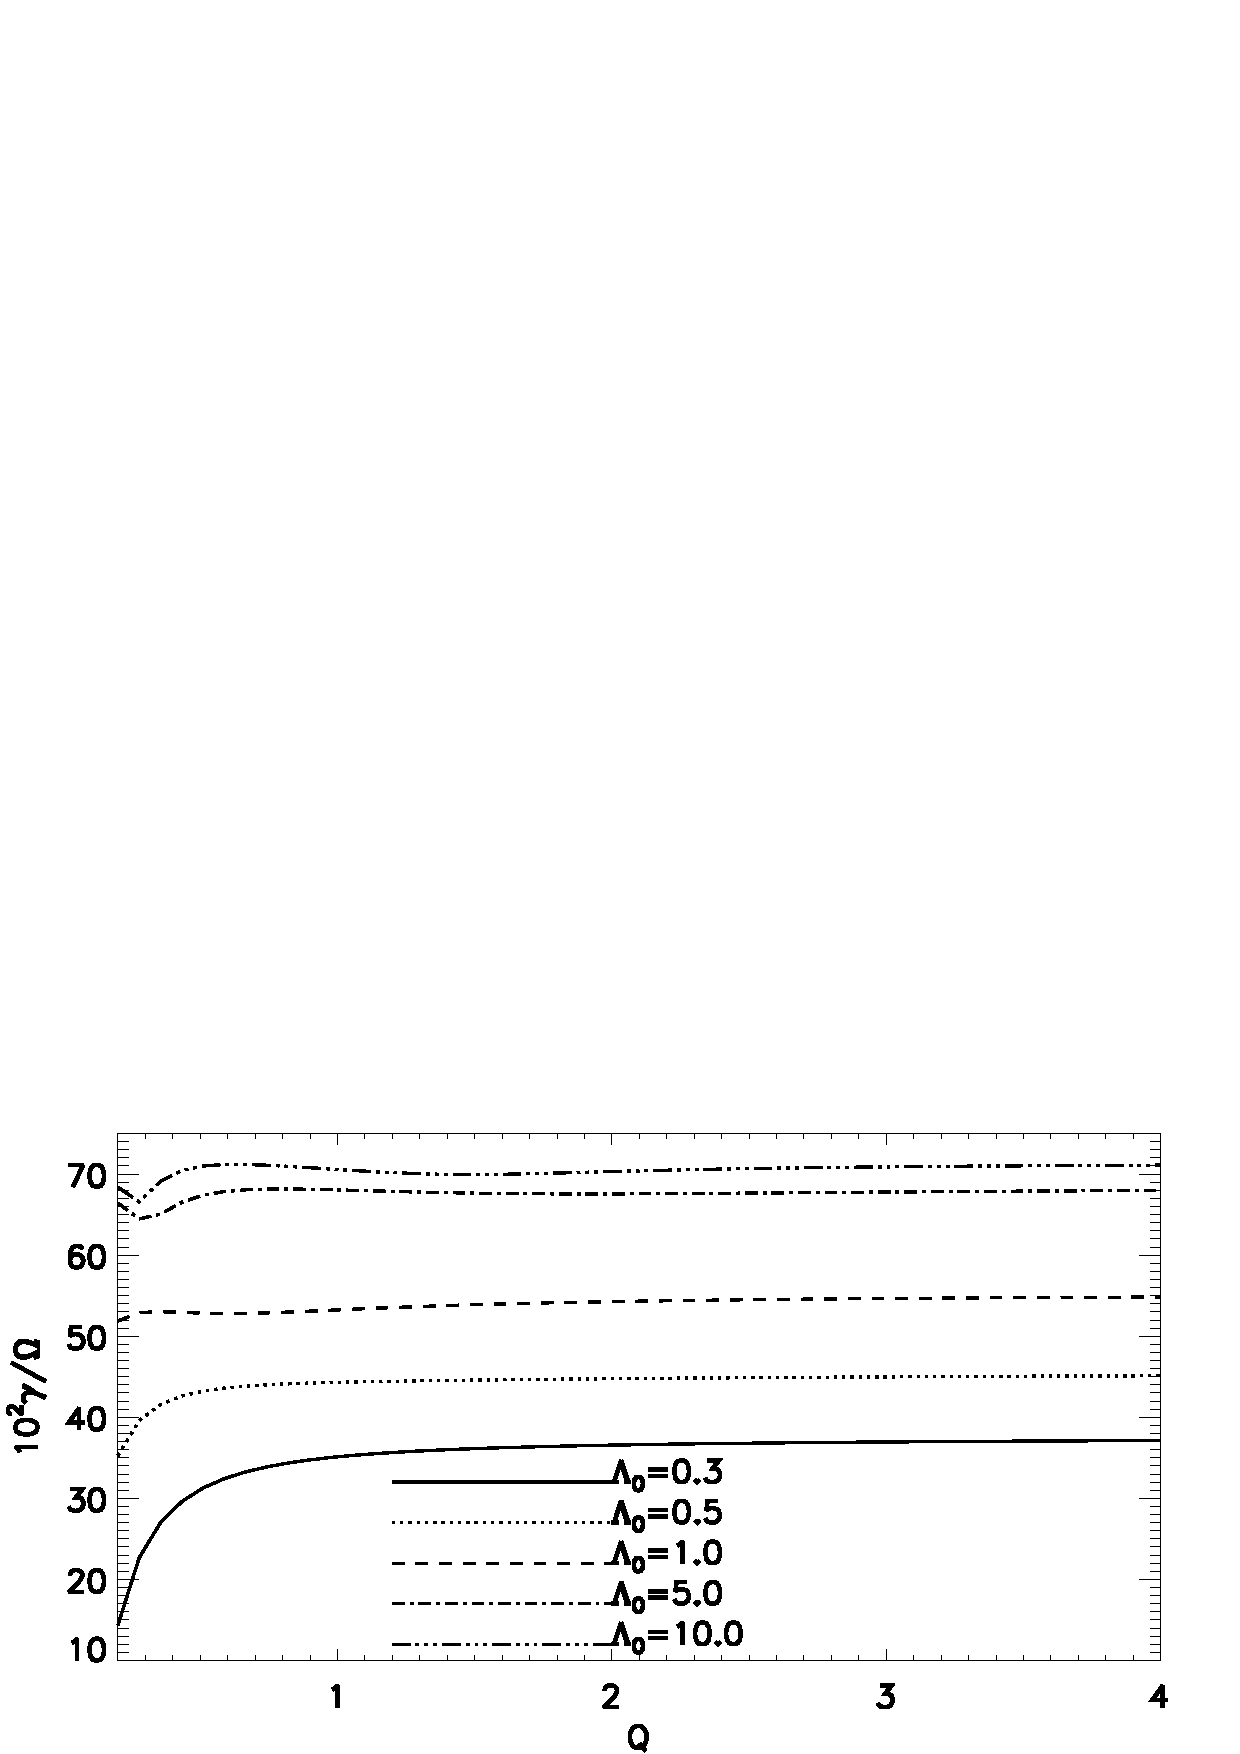
\includegraphics[width=\linewidth]{figures/compare_growth_poly_uniresis}
  \caption{MRI growth rates as a function of $Q$ for mid-planet
    Elsasser numbers $\Lambda_0=0.3$ (solid), $0.5$ (dotted), $1.0$
    (dashed) and $5.0$ (dash-dot).  
    \label{compare_growth_poly_uniresis}}
\end{figure}

% (We find the weak variations in
%$\gamma$ for small $Q$ is associated with a change in the number of
%nodes in the magnetic field perturbation.)
%because $f$ is of order unity for the
%range of $Q$ considered so $\lambda_\mathrm{ideal}$ remain less than
%  unity.
%However, in the resistive limit, the dependence of
%  $\lambda_\mathrm{resis}$ on $f$ (and hence $Q$) is amplified by
%  $\Lambda_0 < 1$.

\cite{sano99} found that for instability to occur the linear mode
dimensional wavelength $\lambda$ should fit inside the disk. That is,   
\begin{align}\label{sano_crit}
  \frac{\lambda}{2H} \equiv
  \mathrm{max}\left(\lambda_\mathrm{ideal},\lambda_\mathrm{resis}\right)\lesssim
  1, 
\end{align}
where the non-dimensional wavelengths are given by 
\begin{align}\label{lambda_ideal}
  \lambda_\mathrm{ideal} = \frac{4\pi}{\sqrt{15}} f v_A =
  \frac{4\pi f}{\sqrt{15\beta\rho}}
\end{align}
in the limit of ideal MHD, and 
\begin{align}\label{lambda_resis}
  \lambda_\mathrm{resis} = \frac{2\pi}{\sqrt{3}}\frac{\eta}{v_A f} =
  \frac{2\pi f}{\Lambda_0}\sqrt{\frac{\rho}{3\beta}} 
\end{align}
%factor pi comes form converting vertical wavenumber to
%wavelength. linear theory works with wavenumber, physical
%interpretation in terms of wavelengths
in the limit of high resistivity. 
%For $\Lambda_0\gtrsim 1$, we find
%the condition $\lambda < 2H$ is well-satisifed throughout most of the
%disk regardless of $Q$.     
The normalized polytropic disk density $\rho$ is weakly dependent
on $Q$ (Fig. \ref{eqm_den}) so self-gravity only affects the
MRI through the factor $f$, which increases with decreasing $Q$ (see
Fig. \ref{plot_fq} in Appendix \ref{appen1}). This suggests that
sufficiently strong self-gravity can stabilize the MRI by making
$ 2H<\lambda $. 
 
%Physically, the
%disk becomes thinner with increasing self-gravity, and the MRI will be
%surpressed when the disk is too thin to accommodate unstable modes. 
%MRI requires
%$\lambda\lesssim 1$, so that the unstable wavelength fits within the
%disk column. As shown in Appendix \ref{appen1}, $f$ increases with the
%strength of self-gravity. This is expected to increase $\lambda$ and
%weaken the MRI.  

%However, $f$ does not vary much for the range of $Q$ considered here. 
In the ideal limit, we find $\lambda < 2H$ throughout most of the disk
for the values of $Q$ considered, so that self-gravity does not affect
growth rates significantly. Fig. \ref{compare_result_lambda10} shows
the magnetic energies for $\Lambda_0=10$ and a range of Toomre $Q$
values. The number of vertical nodes decrease with $Q$, 
%i.e. increasing the strength of vertical self-gravity makes the disk
%unable to accommodate many wavelengths because it becomes thinner. 
i.e. the disk accommodates fewer wavelengths because increasing
vertical self-gravity makes it thinner. 
%As the strength of 
%self-gravity increase, the disk becomes thinner so it can only
%accommodate one wavelength.
Weak variations in growth rates in the ideal limit, seen in 
Fig. \ref{compare_growth_poly_uniresis}, were found to be associated
with changes in the mode character: $\gamma$ decreases
slightly when the mode begins to acquire an additional vertical node as $Q$ is
increased. 

\begin{figure}
  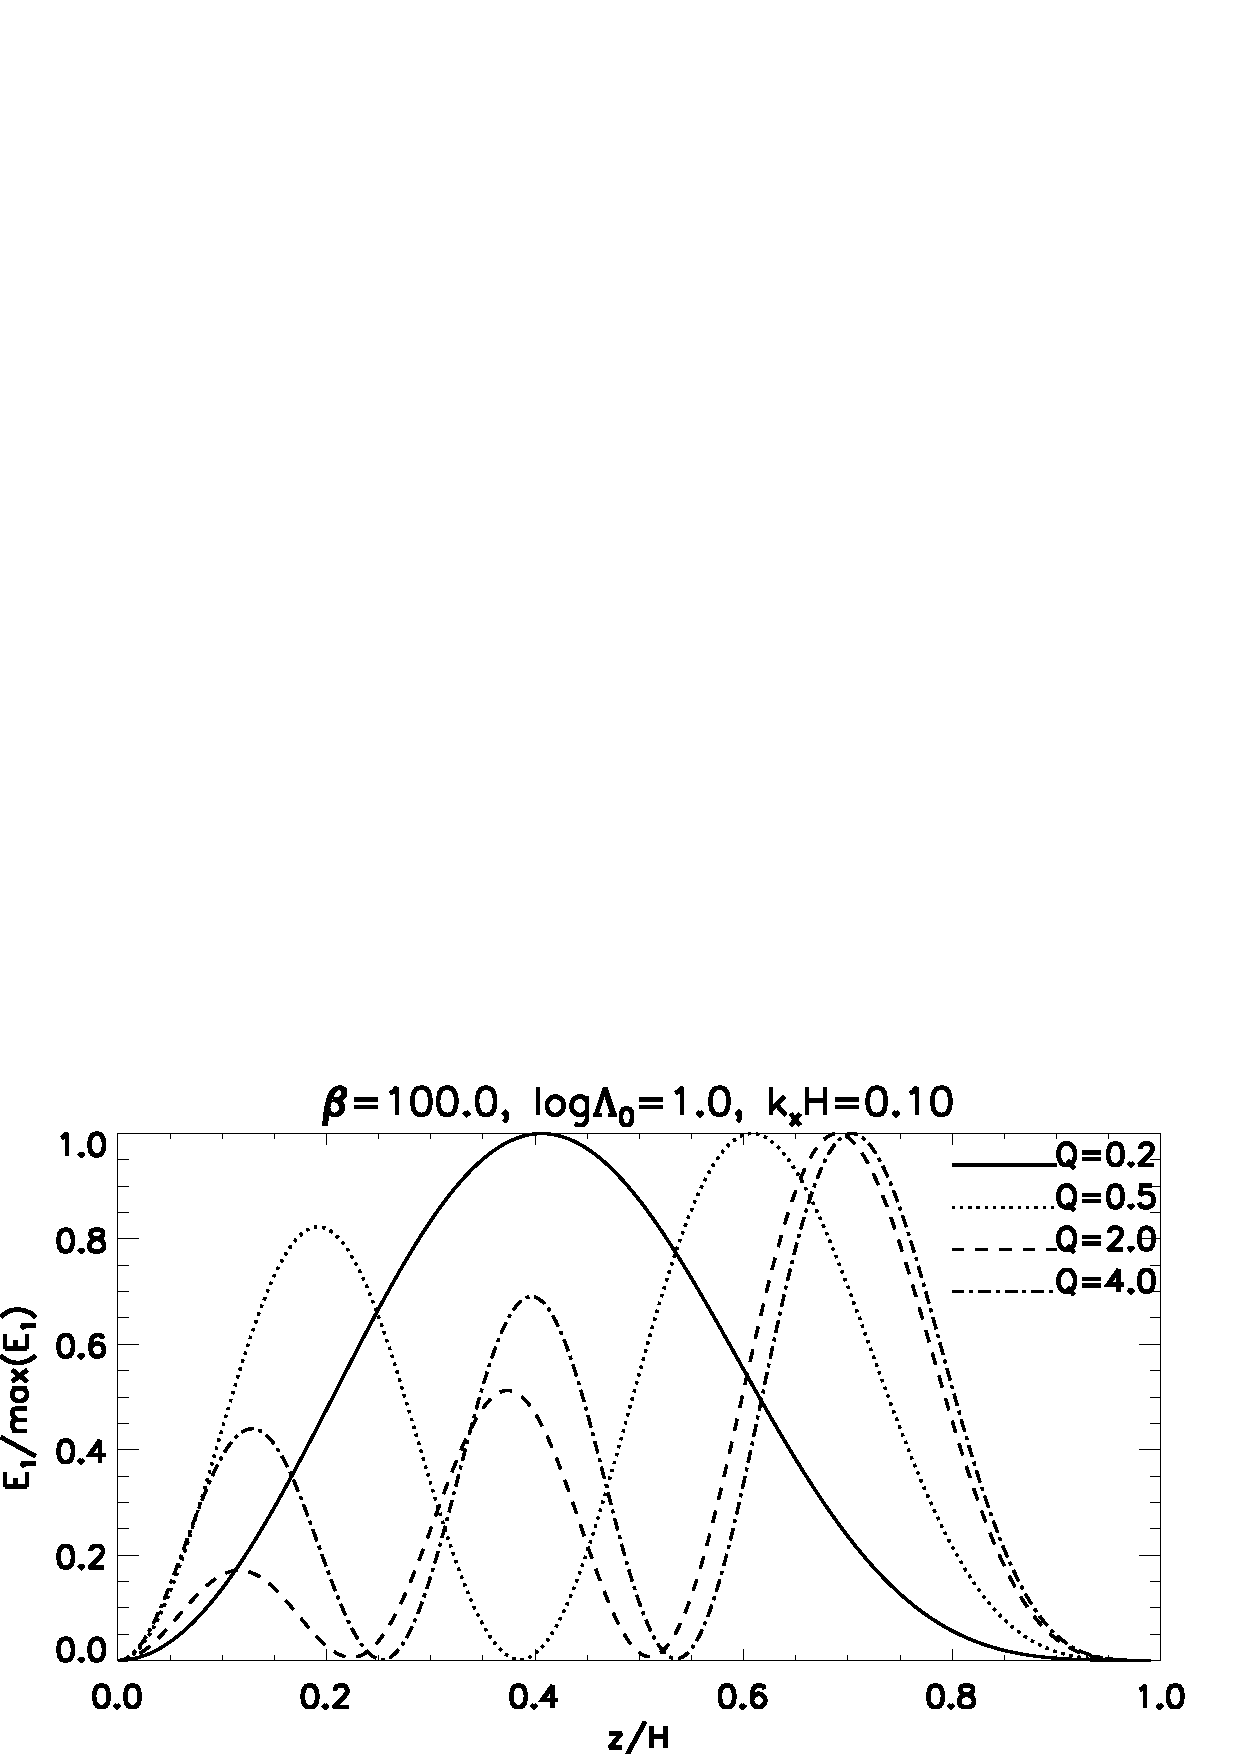
\includegraphics[width=\linewidth]{figures/compare_result_lambda10}
  \caption{Magnetic energies as a function of height, in the limit of
    ideal MHD, for various strengths of self-gravity.   
    \label{compare_result_lambda10}}
\end{figure}

Self-gravity appreciably decreases the MRI growth rates in the
resistive limit. We plot in Fig. \ref{lambda_poly_resis}
Eq. \ref{sano_crit} for $\Lambda_0=0.3$. Even in the
non-self-gravitating disk ($Q=4$) the instability criterion is only
marginally satisfied in the bulk of the disk. As $Q$ decreases, the
Eq. \ref{sano_crit} is violated and the growth rate is dramatically
reduced. This is seen for $Q=0.2$ where $\lambda \geq 2H$ throughout
the disk. (The instability is not completely surpressed since
Eq. \ref{sano_crit} is only an approximation.) Although the function
$f$ does not change significantly for the range of $Q$ considered, the
dependence of $\lambda_\mathrm{resis}$ on $f$ (and therefore $Q$) is
amplified by the denominator $\Lambda_0<1$ in the resistive case. For resistively cases
we find no nodes in the magnetic energy $E_1$ except at end points,
i.e. only the longest wavelength survives Ohmic dissipation. 


%only one wavelength. no nodes except endpoints.    


%although $f$ does not vary significantly, the dependence of
%$\lambda_\mathrm{resis}$ on $f$ is amplified by $\Lambda_0<1$ in the
%denominator of Eq. \ref{lambda_resis}. Even in the 


\begin{figure}
  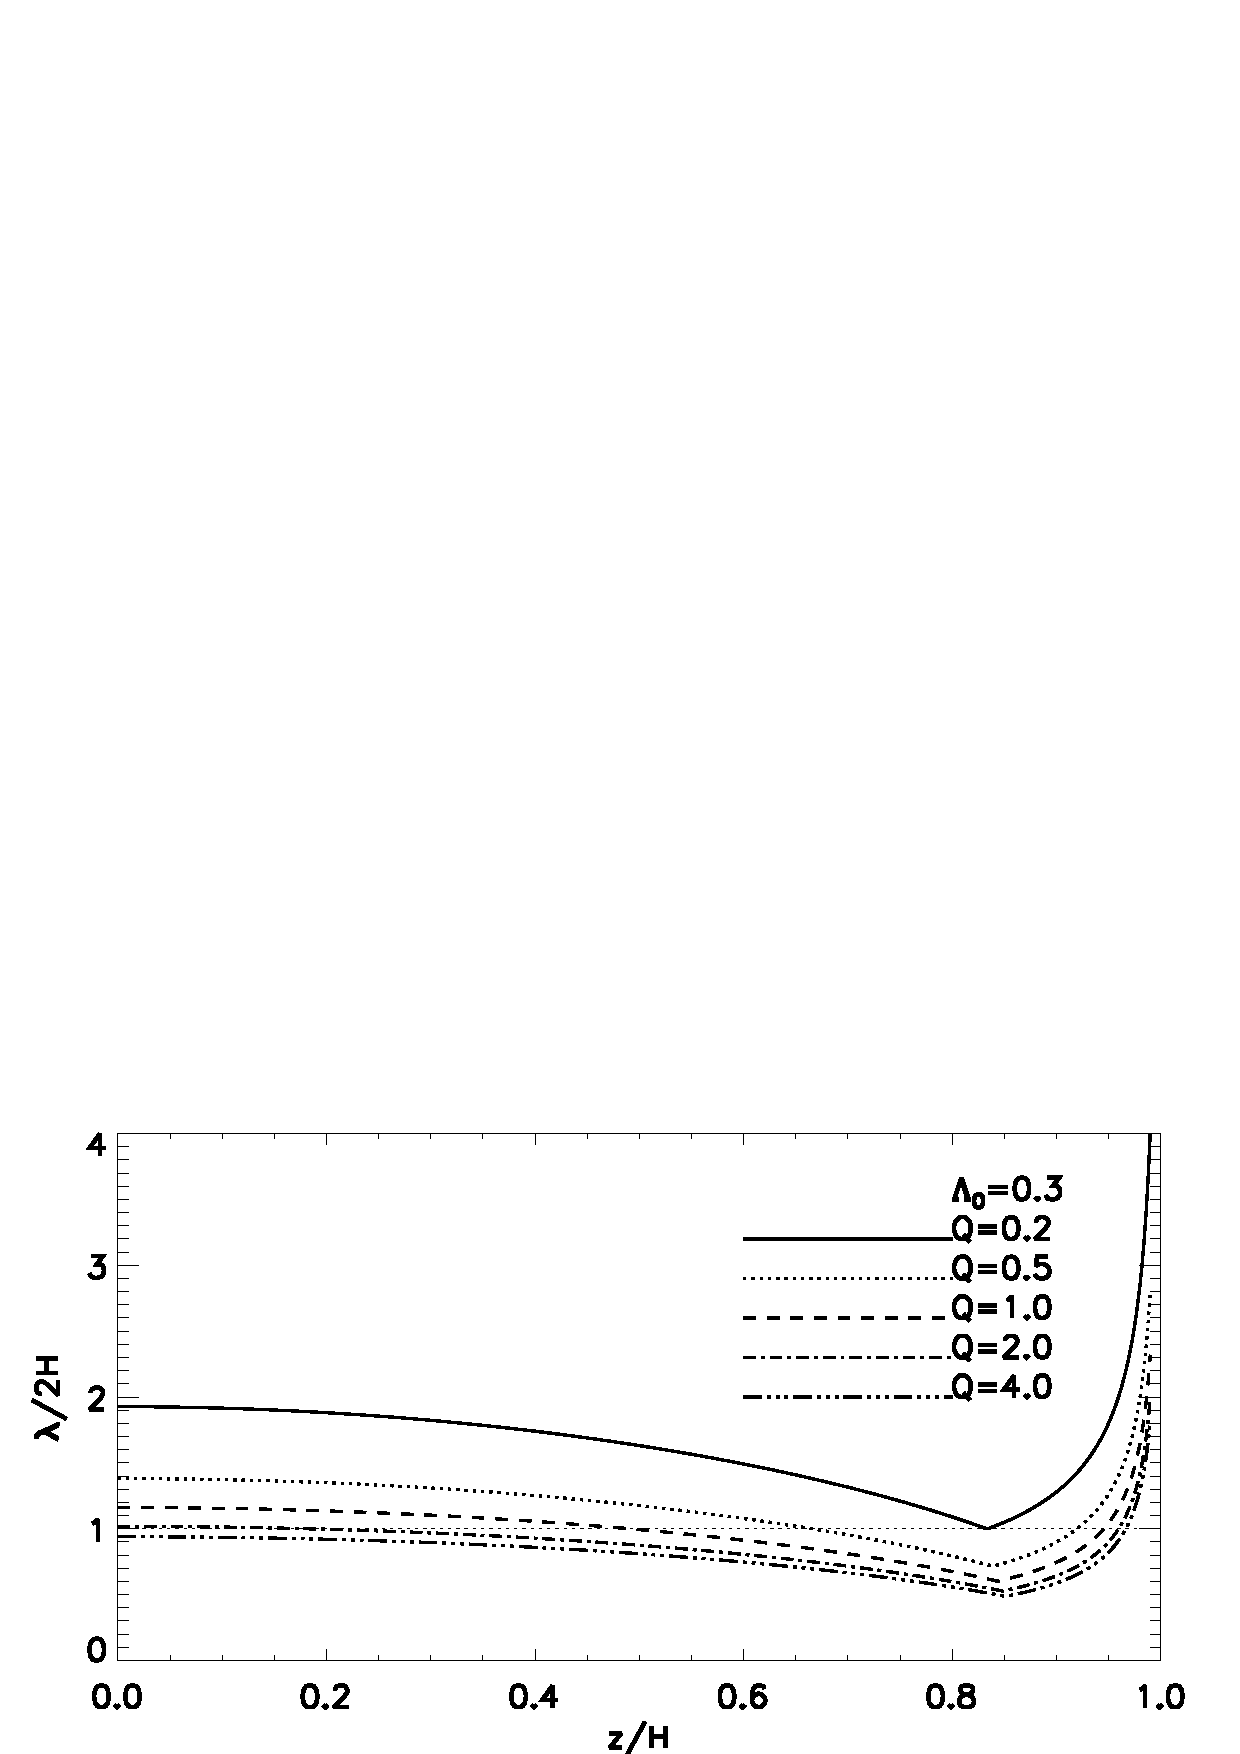
\includegraphics[width=\linewidth]{figures/lambda_poly_uniresis}
  \caption{Approximate wavelengths of the most unstable resistive MRI modes as given by
    Eq. \ref{sano_crit}---\ref{lambda_resis}, normalized by the 
    disk thickness, as a function of height for a range of Toomre $Q$
    values.  
    \label{lambda_poly_resis}}
\end{figure}


\subsection{Resistive MRI in self-gravitating polytropic disks with layered
  resistivity} 
Here we consider disks with mid-plane Elsasser number $\Lambda_0=0.1$
and layered resistivity with $A=10^2$. We use $k_x=0.1$ as before.  
Fig. \ref{poly_layer} compares the magnetic 
energies for $Q=0.2,\,1$ and $4$. They have similar growth rates, $\gamma/\Omega
= 0.53,\,0.64$ and $0.66$, respectively. In the non-self-gravitating
limit ($Q=4$), the MRI is effectively surpressed for $z\lesssim0.5H$, whereas
in the massive disk ($Q=0.2$) the mode occupies a wider vertical
extent because its wavelength (in units of $H$) is larger. This
suggests that in massive disks the MRI is not well localized to the
active layer, as the instability takes on a more global character
compared to non-self-gravitating disks.        
%d is not as well localized

\begin{figure}
  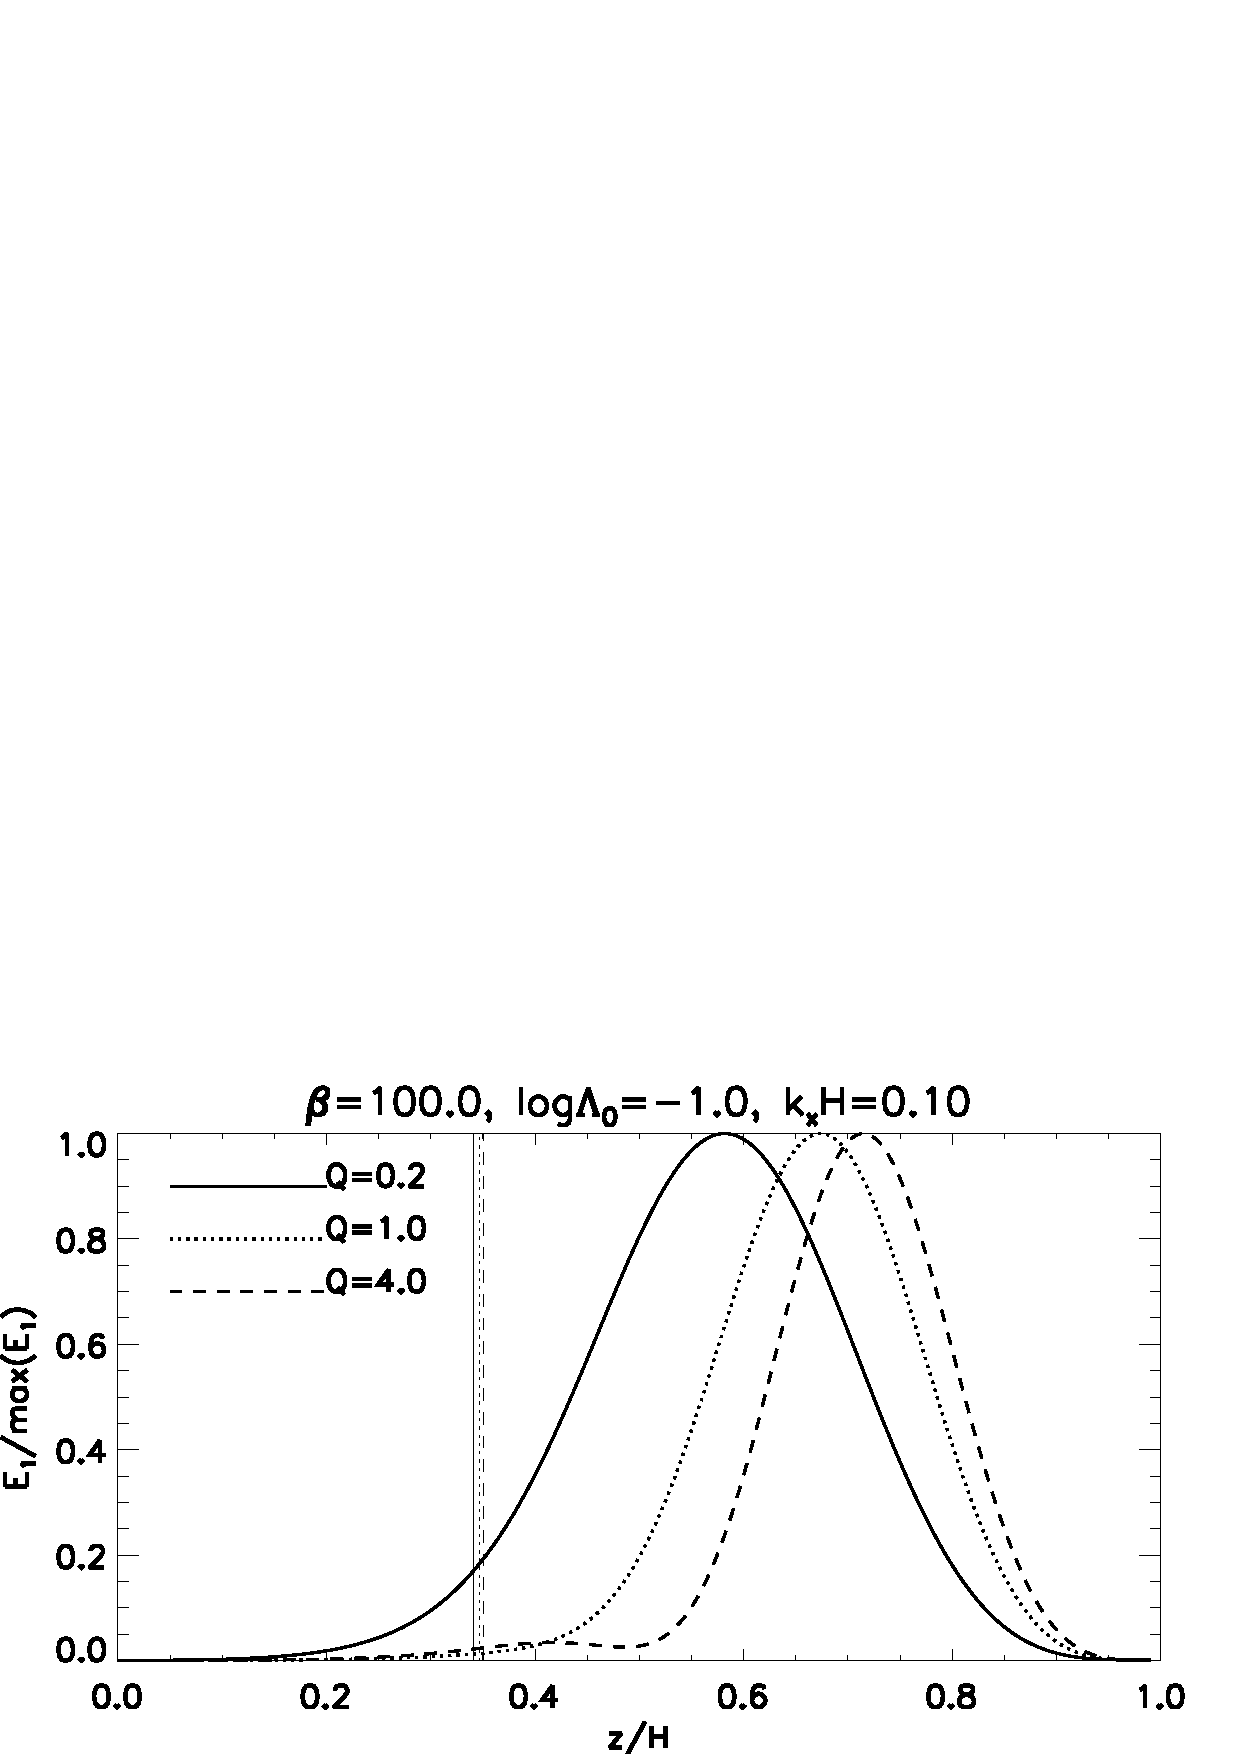
\includegraphics[width=\linewidth]{figures/compare_results_poly_layer_amp100}
  \caption{Magnetic energies as a function of height, for layered polytropic disks with
    such that the conductivity increases by a 
    factor of $10^2$ in going from the mid-plane to the upper disk
    boundary. The vertical lines indicate $\Lambda=1$ for each value
    of $Q$.
    \label{poly_layer}}
\end{figure}

%\subsection{GI in magnetized isothermal disks with uniform
%  resistivity} 


%\subsection{GI in magnetized isothermal disks with layered
%  resistivity} 

\subsection{Non-zero radial wavenumbers}  
As remarked above, for $k_xH\ll 1$ the most unstable linear mode is
the incompressible MRI with vanishing density and potential 
perturbtions. For self-gravity to play a role in the linear
pertubrations we consider $k_xH \neq 0$ and also an isothermal
disk. From \cite{mamat10}, we expect GI to set in
for $Q\lesssim 0.2$. 
%We expect modes associated with GI have $k_x\sim 1/H$, for modes
%with smaller $k_x$ are stabilized by rotation and 
 
In Fig. \ref{compare_growth_varQ} we plot the growth rate of 
unstable modes in disks with uniform resistivity and varying $Q$.  
The appearence of a bump at $k_xH\sim1$ for $Q< 0.2$ signifies GI. 
%We checked that the perturbed energy is dominated
%by gravitational energy.   
%Because the most unstable MRI mode occurs at $k_xH=0$ while the most
%unstable GI mode occurs at $k_xH\sim1$, 
We expect a sufficiently massive magnetized disk to undergo both MRI
at long radial lengthscales ($k_xH\ll 1$) and GI at intermediate
radial lengthscales ($k_xH\sim 1$). However, unless the system
parameters are finely tuned, the MRI and GI modes do not grow
at the same rate. For example, at $Q=0.17$ GI is expected but
increasing it slightly to $Q=0.2$, MRI dominates. This is largely due
to promoting GI with decreasing $Q$, although lowering $Q$ also
stabilizes the MRI. 

\begin{figure}
  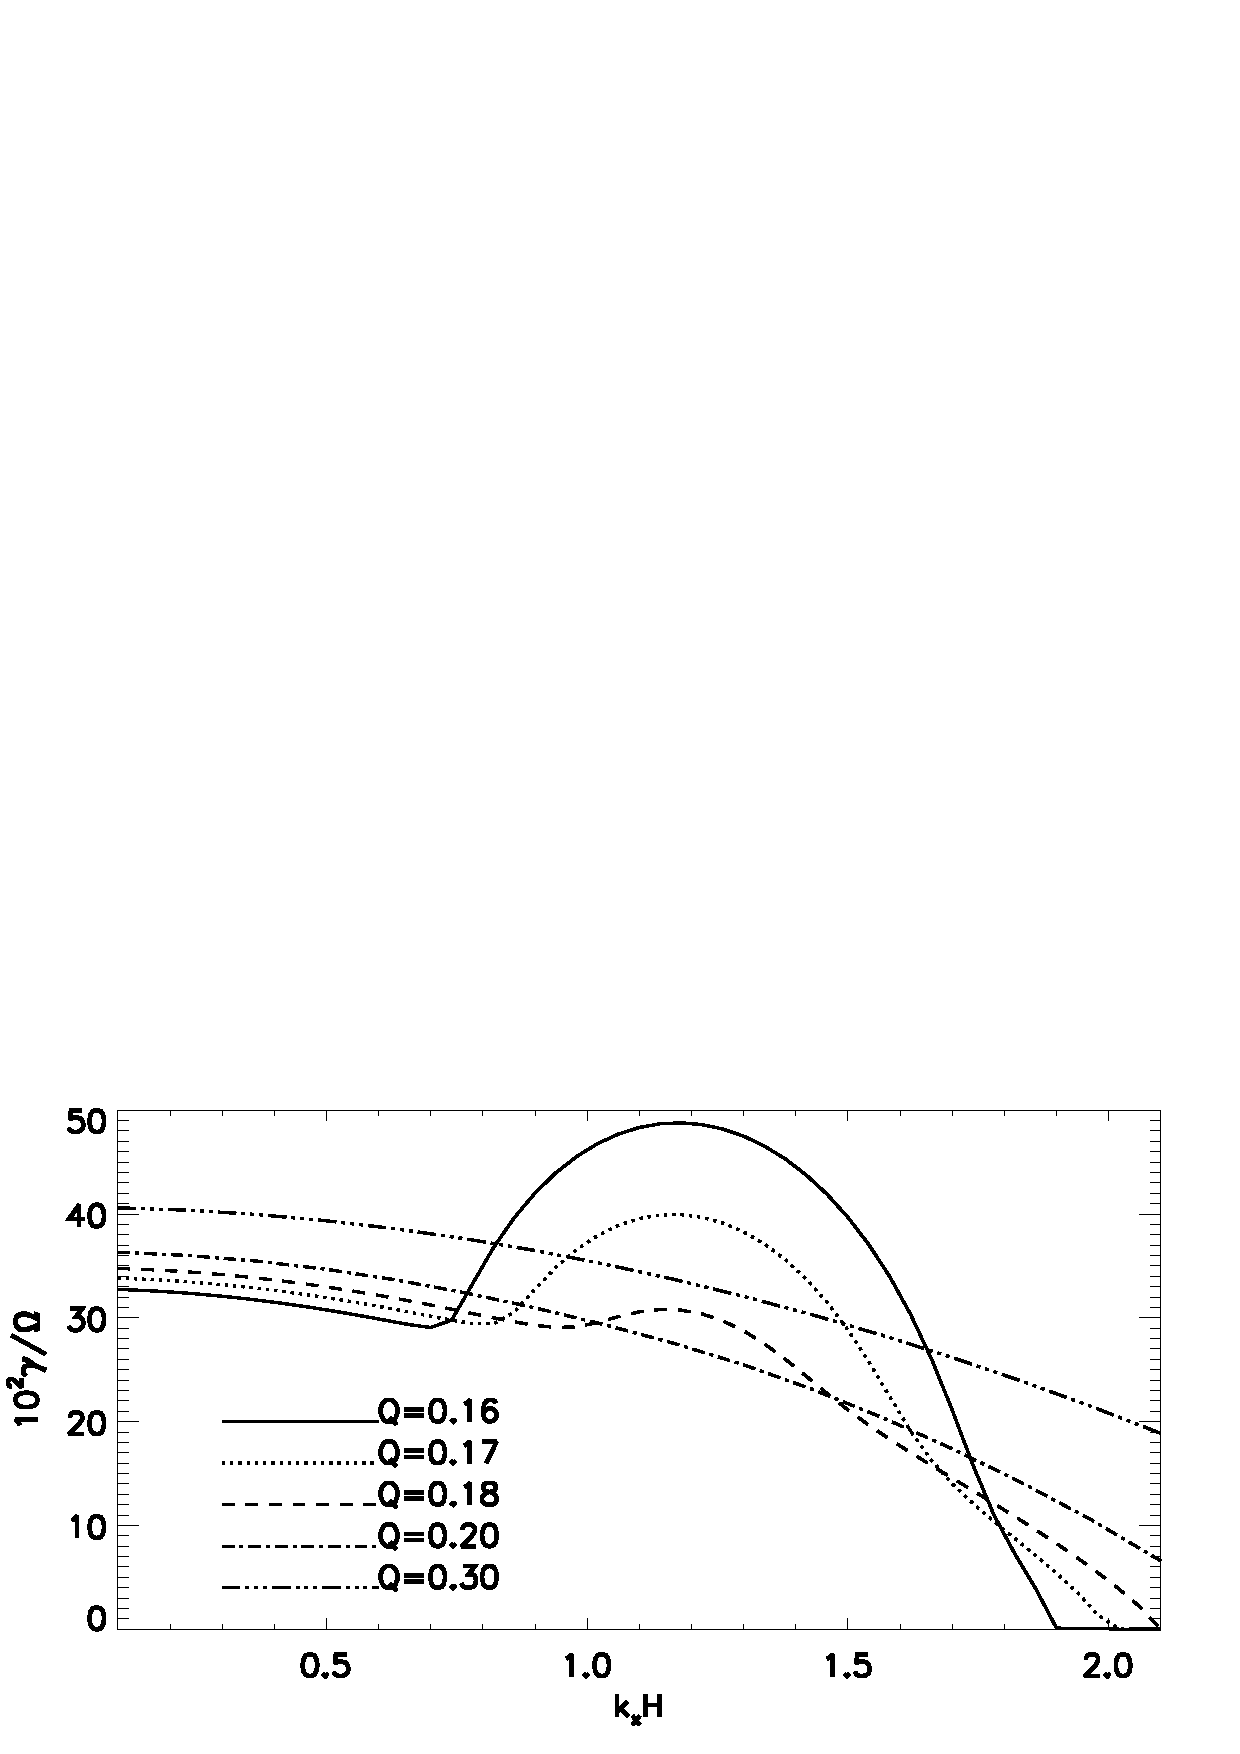
\includegraphics[width=\linewidth]{figures/compare_growth_varQ}
  \caption{Linear growth rates as a function of horizontal wavenumber
    $k_x$ in a resistive disk with $\Lambda_0=0.1$ and varying
    strengths of self-gravity. 
    \label{compare_growth_varQ}}
\end{figure}

%Strictly speaking, given a set of disk parameters, one is only
%concerned with the most unstable linear mode. 


%The plot indicates the peak GI growth rate is
%$\gamma\sim 0.3\Omega$.  



\begin{figure}
  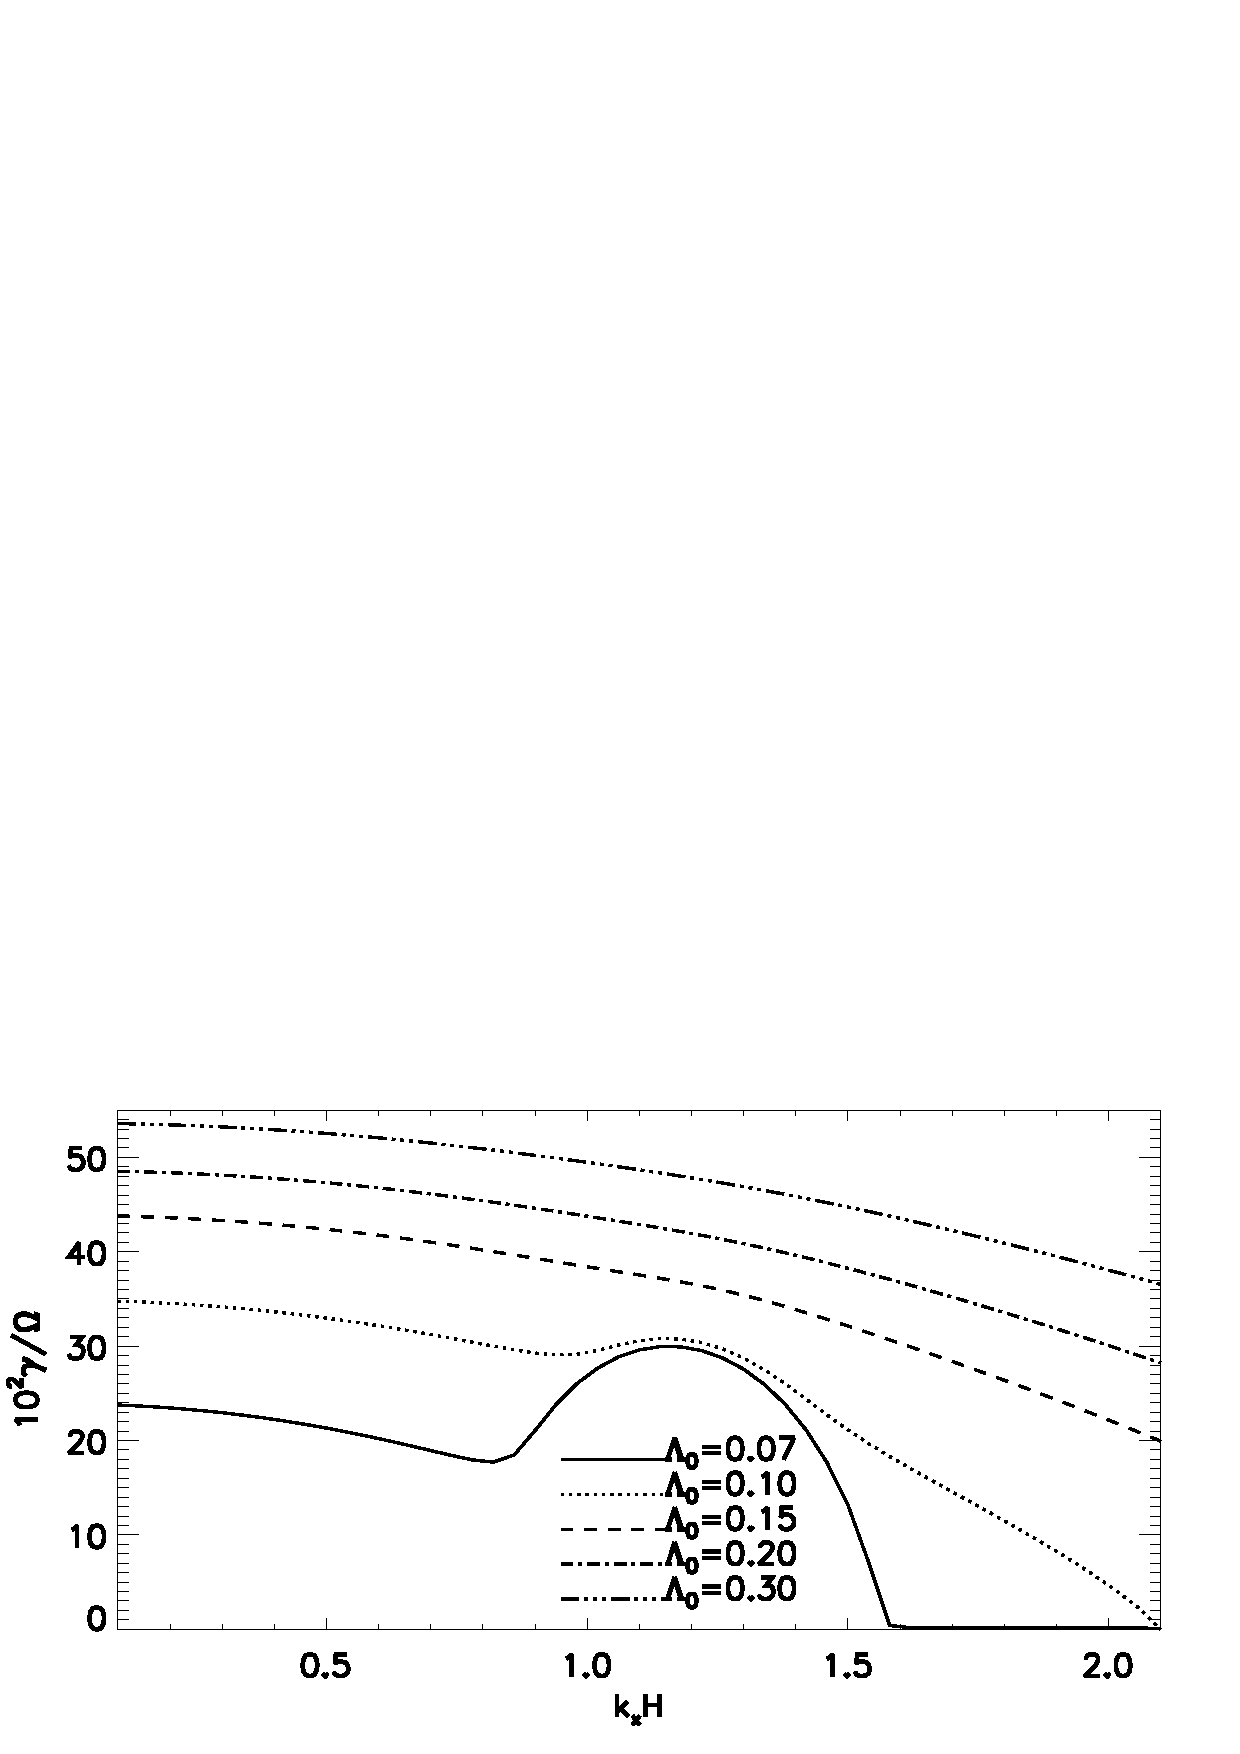
\includegraphics[width=\linewidth]{figures/compare_growth_varLam}
  \caption{Linear mode growth rates as a function of horizontal wavenumber
    $k_x$ in a self-gravitating disk with $Q=0.18$ and uniform resitivity 
     as measured by the mid-plane Elsasser number $\Lambda_0$.
    \label{compare_growth_varLam}}
\end{figure}


\begin{figure}
  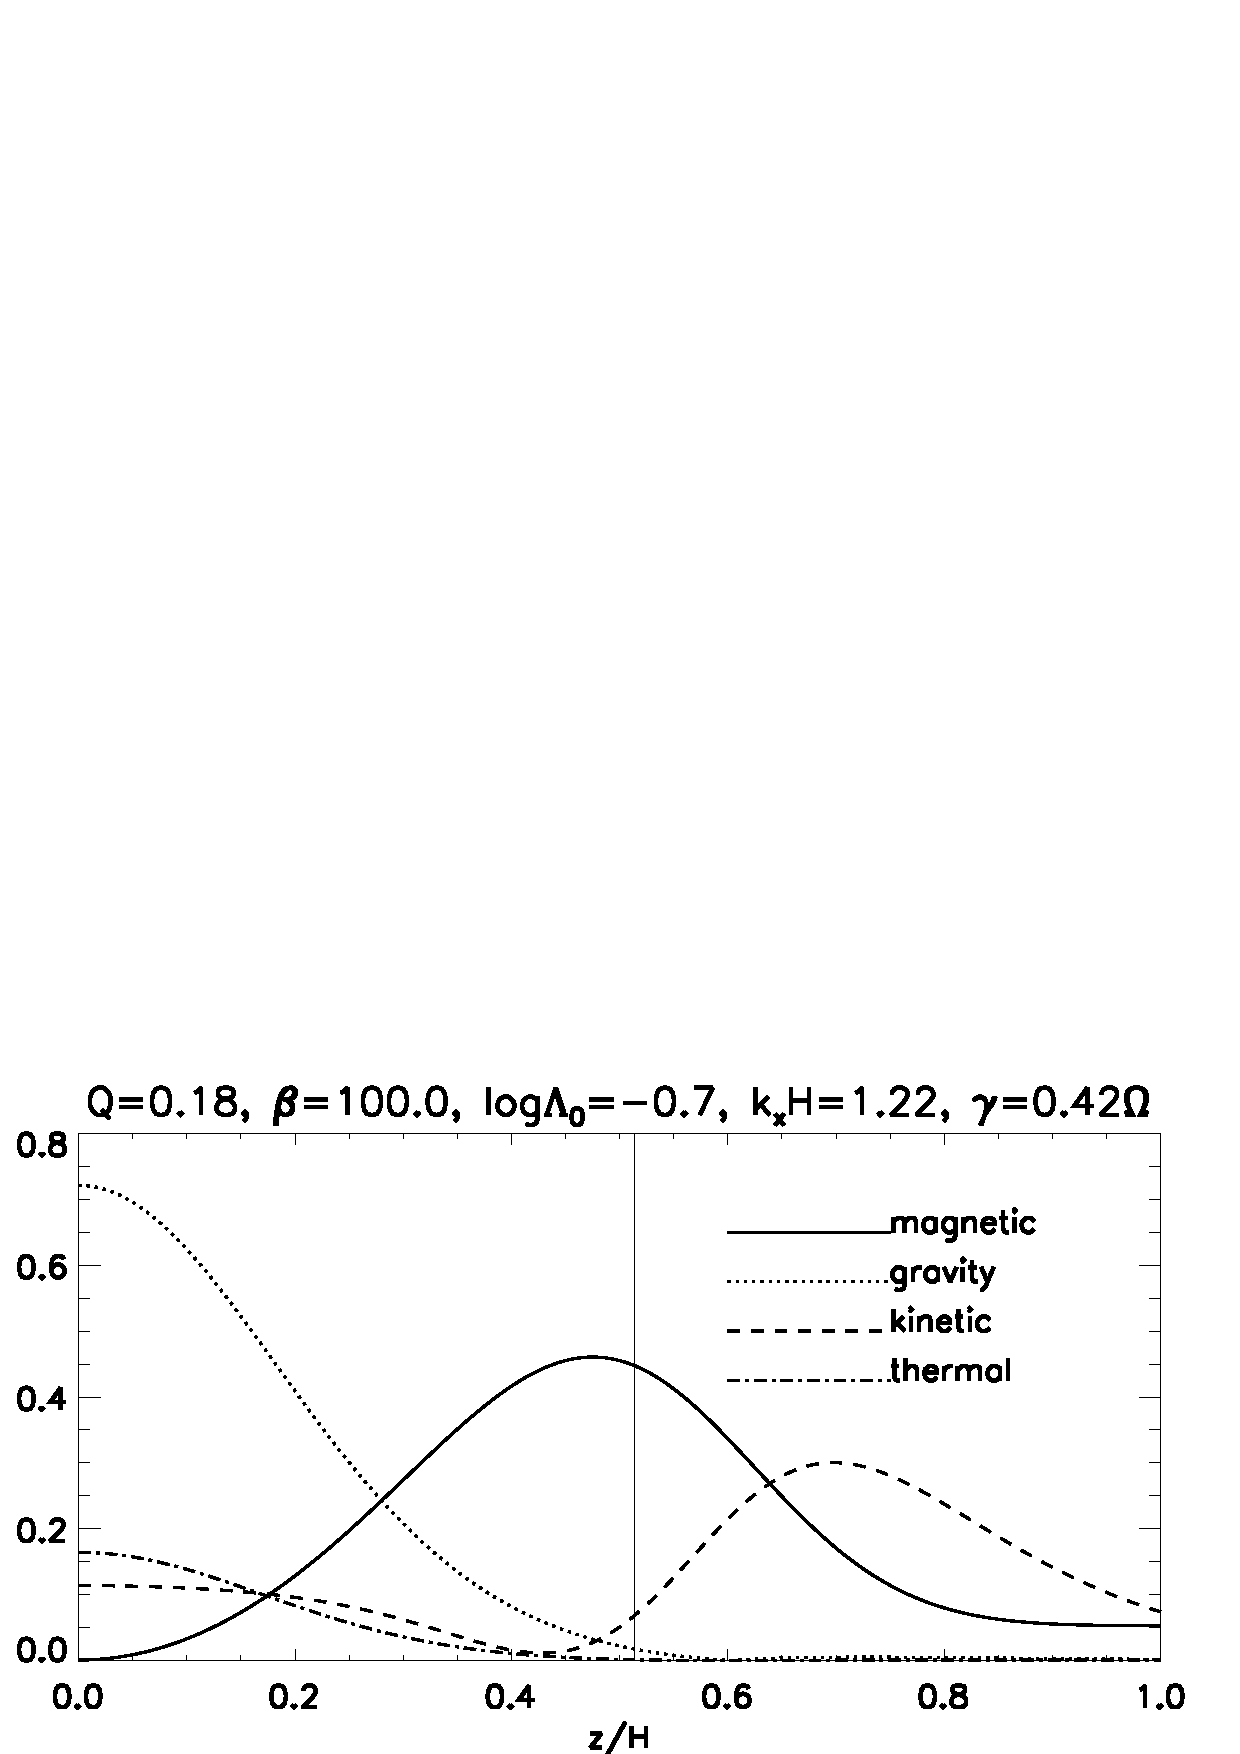
\includegraphics[width=\linewidth]{figures/result_Q0d18_lamda0d2}
  \caption{Perturbation energies for a linear mode in a
    self-gravitating disk ($Q=0.18$) with uniform resistivity (such
    that $\Lambda_0=0.2$). 
    The mangetic
    ($E_m$, solid), gravitational ($E_k$, dotted ), kinetic ($E_k$,
    dashed) and thermal ($E_t$, dash-dot) energies are normalized by
    the maximum of the total energy.  
    \label{result_Q0.18_lambda0.2}}
\end{figure}


%to get compressibility effects, need kx non zero 
%technically not fastest, but still pretty fast 


%\subsection{Influence of vertical magnetic field on gravitational
%  instability} 
